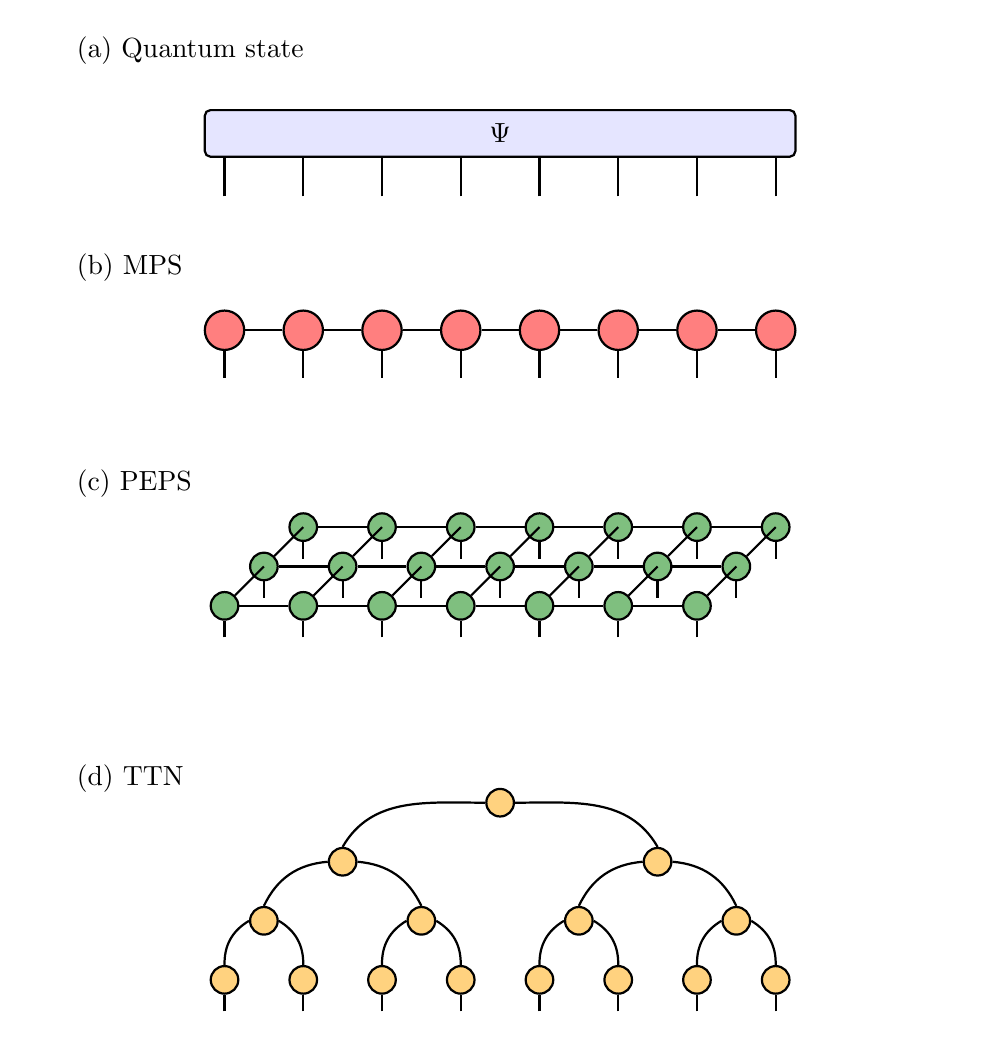
\begin{tikzpicture}[
    index/.style = {thick},
    mps tensor/.style = {circle, draw, thick, fill=Red, fill opacity=0.5, minimum size=0.5cm, inner sep=0pt},
    peps tensor/.style = {circle, draw, thick, fill=Green, fill opacity=0.5, minimum size=0.35cm, inner sep=0pt},
    ttn tensor/.style = {circle, draw, thick, fill=Orange, fill opacity=0.5, minimum size=0.35cm, inner sep=0pt}
    ]
    % Generic quantum state
    \node[
    rectangle,
    minimum width=7.5cm,
    draw,
    thick,
    inner sep=5pt,
    rounded corners=2pt,
    fill=Blue,
    fill opacity=0.1,
    font=\normalsize,
    text=black,
    text opacity=1
    ] (psi) at (0, 0) {$\ket{\Psi}$};
    \foreach \n in {-3.5, -2.5, ..., 3.5} {
        \draw[index] (\n, -0.8) -- (\n, -0.8 |- psi.south);
    }

    % MPS
    \begin{scope}[yshift=-2.5cm, xshift=-3.5cm]
        \foreach \n in {0, ..., 7} {
            \node[mps tensor] (mps \n) at (\n, 0) {};
            \draw[index] (\n, -0.6) -- (\n, -0.6 |- mps \n.south);
        }
        \foreach \n in {0, ..., 6} {
            \pgfmathtruncatemacro{\m}{\n + 1}
            \draw[index] (mps \n.east) -- (mps \m.west);
        }
    \end{scope}

    % PEPS
    \begin{scope}[yshift=-6cm, xshift=-3.5cm]
        \foreach \y/\n in {0/0, 0.5/1, 1/2} {
            \foreach \x in {0, ..., 6} {
                \node[peps tensor] (peps \x \n) at (\x + \y, \y) {};
                \draw[index] (\x + \y, \y-0.4) -- (\x + \y, \y-0.4 |- peps \x \n.south);
            }
            \foreach \x in {0, ..., 5} {
                \pgfmathtruncatemacro{\w}{\x + 1}
                \draw[index] (peps \x \n.east) -- (peps \w \n.west);
            }
        }
        \foreach \n in {1, 2} {
            \pgfmathtruncatemacro{\m}{\n-1}
            \foreach \x in {0, ..., 6} {
                \draw[index] (peps \x \n.center) -- (peps \x \m.north east);
            }
        }
    \end{scope}

    % TTN
    \begin{scope}[yshift=-10.75cm, xshift=-3.5cm]
        % level 0
        \foreach \n in {0, ..., 7} {
            \node[ttn tensor] (ttn 0 \n) at (\n, 0) {};
            \draw[index] (\n, -0.4) -- (\n, -0.4 |- ttn 0 \n.south);
        }

        % level 1
        \foreach \n in {0, ..., 3} {
            \pgfmathsetmacro{\x}{2 * \n + 0.5}
            \node[ttn tensor] (ttn 1 \n) at (\x, 0.75) {};
        }

        % level 2
        \foreach \n in {0, 1} {
            \pgfmathsetmacro{\x}{4 * \n + 1.5}
            \node[ttn tensor] (ttn 2 \n) at (\x, 1.5) {};
        }

        % level 3
        \node[ttn tensor] (ttn 3) at (3.5, 2.25) {};

        % indices
        \foreach \n in {0, ..., 3} {
            \pgfmathtruncatemacro{\a}{2 * \n}
            \pgfmathtruncatemacro{\b}{2 * \n + 1}
            \draw[index] (ttn 0 \a.north) edge[bend left ] (ttn 1 \n.west);
            \draw[index] (ttn 0 \b.north) edge[bend right] (ttn 1 \n.east);
        }
        \foreach \n in {0, 1} {
            \pgfmathtruncatemacro{\a}{2 * \n}
            \pgfmathtruncatemacro{\b}{2 * \n + 1}
            \draw[index] (ttn 1 \a.north) edge[bend left ] (ttn 2 \n.west);
            \draw[index] (ttn 1 \b.north) edge[bend right] (ttn 2 \n.east);
        }
        \draw[index] (ttn 2 0.north) edge[out=60, in=180] (ttn 3.west);
        \draw[index] (ttn 2 1.north) edge[out=120, in=0] (ttn 3.east);
    \end{scope}

    % Labels
    \node[anchor=south west] at (-5.5, 0.75) {(a) Quantum state};
    \node[anchor=south west] at (-5.5, -2)   {(b) MPS};
    \node[anchor=south west] at (-5.5, -4.75)   {(c) PEPS};
    \node[anchor=south west] at (-5.5, -8.5) {(d) TTN};

    % for centering
    \path (-6, 0) -- (6, 0);
\end{tikzpicture}

